%! Author = sutingchen
%! Date = 2023/10/18

\titledquestion{Generate a binary tree}

\begin{parts}
    \part[4] Given the in-order and pre-order traversal of a binary tree T are \textbf{ECFBDGA} and \textbf{ABCEFDG} respectively.\\
    Draw the tree T.\\
    \begin{solution} \\
        %\vspace{15em}
        \begin{center}
            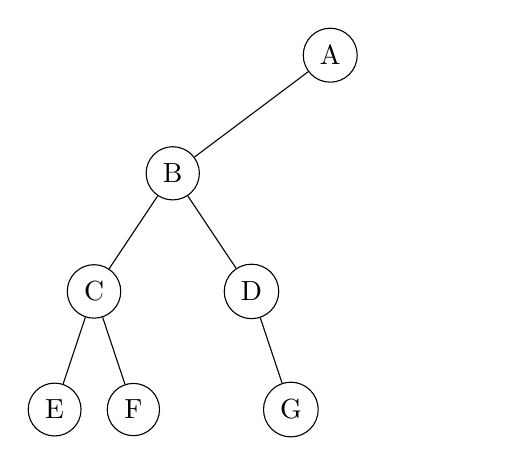
\begin{tikzpicture}[level distance=1.5cm,
                    level 1/.style={sibling distance=4cm},
                    level 2/.style={sibling distance=2cm},
                    level 3/.style={sibling distance=1cm},
                    every node/.style = {draw, circle}]
                \node {A}
                child { node {B}
                        child { node {C}
                                child { node {E} }
                                child { node {F} }
                            }
                        child { node {D}
                                child { edge from parent[draw=none] }
                                child { node {G} }
                            }
                    }
                child { edge from parent[draw=none] };
            \end{tikzpicture}
        \end{center}
    \end{solution}
    \vspace{2cm}
    \part[4] Given the in-order and post-order traversal of a binary tree T are \textbf{EBDAHCGF} and \textbf{EDBHFGCA} respectively.\\
    Draw the tree T.\\
    \begin{solution} \\
        %\vspace{15em}
        \begin{center}
            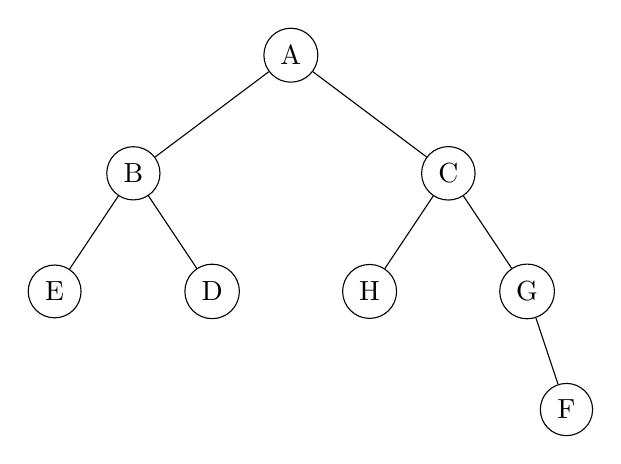
\begin{tikzpicture}[level distance=1.5cm,
                    level 1/.style={sibling distance=4cm},
                    level 2/.style={sibling distance=2cm},
                    level 3/.style={sibling distance=1cm},
                    every node/.style = {draw, circle}]
                \node {A}
                child { node {B}
                        child { node {E} }
                        child { node {D} }
                    }
                child { node {C}
                        child { node {H} }
                        child { node {G}
                                child { edge from parent[draw=none] }
                                child { node{F} }
                            }
                    };
            \end{tikzpicture}
        \end{center}
    \end{solution}
    % \vspace{2cm}
    \pagebreak
    \part[2] Given the pre-order and post-order traversal of a binary tree T, can you decide the tree T? If yes, please describe an algorithm to construct T; if no, please provide a counterexample.\\
    \begin{solution} \\
        %\vspace{20em}
        Knowing the pre-order and the post-order, we can construct the tree. \\
        \begin{enumerate}
            \item The first element in the pre-order and the last element in the post-order is the same,
                  which is the root. Remove it.
            \item The second element in the pre-order is the first children of the first element,
                  thus in the post-order elements in front of it form a subtree.
            \item Regard the subtree as a new tree and repeat the operations above.
            \item If facing with the elements shares the same position in pre-order and post-order,
                  this element is a leaf. For example, if ACB is the pre-order and ABC is the post-order,
                  A will be the leaf of the tree. Remove it.
        \end{enumerate}

    \end{solution}
\end{parts}